\documentclass[conference]{IEEEtran}
\usepackage{amsmath,amssymb}
\usepackage{graphicx}
\usepackage{booktabs}
\usepackage{url}
\usepackage[hidelinks]{hyperref}
\graphicspath{{figures/}}

\begin{document}

\title{SENTINEL-HTN: Personalized, Uncertainty-Aware Early Warning of Emerging Hypertension from a Single Wrist Strap}

% TODO: complete team members and affiliation before submission.
\author{\IEEEauthorblockN{Ibrahim Dammak and team}
\IEEEauthorblockA{BioVance AIoT Challenge --- IEEE EMBS Tunisia\\
Code: \url{https://github.com/IbrahimDammak/sentinel-htn}}}

\maketitle

\begin{abstract}
Hypertension develops silently while blood pressure (BP) is measured only episodically. SENTINEL-HTN is an AIoT system in which one wrist strap supplies nightly heart rate (HR), heart-rate variability, sleep and activity. It learns each wearer's baseline and combines channels with literature-informed, reliability-adjusted weights. It tracks persistent drift with CUSUM, persistence rules and a Kalman trend, and estimates the risk of reaching a home-BP hypertension reference within 26 weeks. Its output is a warning, ``insufficient evidence'' or ``poor-quality data''. We calibrated our simulator against 71 real Fitbit users (LifeSnaps), matching their means, between-person spreads, day-to-day noise and autocorrelation. On held-out people over three seeds, the system reached an AUROC of $0.621\pm0.014$ and an AUPRC of $0.120\pm0.020$, above level-only, cuff-only and equal-weight versions in every seed, with an expected calibration error of 0.006 at 0.41 alarms per non-converter person-year. It warned 32\% of converters at least 30 days ahead, against 25\% for random alarms at the same rate (above chance in every seed), but not 90 days ahead. An uncalibrated simulator had overstated this advantage, and the weighting gain rests mainly on the literature prior, so real labels must confirm both. On the real cohort the system issued no warnings over 8.3 person-years (95\% upper bound 0.36) and abstained in 23\% of weeks. Weighting reduced real weekly noise from 0.52 to 0.41. Abstention was five times higher in the darkest skin-tone tercile. We report these limits and release reproducible code.\n\end{abstract}

\begin{IEEEkeywords}
hypertension, wearables, photoplethysmography, personalization, change detection, calibration, abstention, real-world validation
\end{IEEEkeywords}

\section{Introduction}
Hypertension is a leading modifiable cardiovascular risk factor with a silent onset. Its detection relies on intermittent office measurements, although out-of-office BP is more prognostic: in 59,124 patients, 24-h systolic BP was associated with mortality with a hazard ratio of 1.41 per standard deviation, against 1.18 for clinic BP \cite{staplin2023}. Converting wearable signals into BP has not earned clinical trust. The European Society of Hypertension does not recommend cuffless devices for diagnosis or management \cite{esh2022}, its validation recommendations require dedicated tests of calibration, device position, treatment, exercise and awake--asleep changes \cite{stergiou2023}, and a 2026 American Heart Association statement judged such devices not yet adequately vetted \cite{aha2026}. In the Aurora project (1,125 participants), no waveform model beat the calibration cuff reading plus time of day \cite{mukkamala2023}, and a PTT device tracked a 7.4\,mmHg change as 1.8\,mmHg \cite{derendinger2024}. The first regulator-cleared alternative avoids BP estimation: Apple's Hypertension Notification Feature classifies 30-day PPG windows, with a sensitivity of 41.2\% and a specificity of 92.3\% \cite{k250507}, and modelling suggests that 58.8\% of people with undiagnosed hypertension would receive no alert \cite{cohen2026}.

The BioVance challenge asks whether longitudinal data can identify an individual's transition toward hypertension risk before clinical detection, with personalization, temporal reasoning, context awareness, robustness and principled abstention (RQ1--RQ6). SENTINEL-HTN uses one strap and outputs no BP number. Its design was selected by a citation-audited comparison of six candidate architectures. It makes three contributions:
\begin{enumerate}
\item an interpretable Learn--Detect--Predict--Warn pipeline with a three-state output;
\item an evaluation that counts abstention as a miss, reports alarms per non-converter person-year, and compares early detection with level-only and cuff-only baselines and a random-alarm floor;
\item calibration of the simulator against real wearable data, plus a label-free real-world transfer test.
\end{enumerate}

\section{Related Work}
\emph{Wearable precursors.} In 232,587 adults, low 10-s ECG heart-rate variability was associated with incident hypertension (hazard ratio 1.58) \cite{kang2022}. In HELIUS, however, baroreflex sensitivity predicted it but SDNN and RMSSD did not \cite{bouwmeester2025}. In All of Us, each additional 1,000 daily steps was associated with lower odds (OR 0.92) \cite{master2022} and irregular sleep with higher odds (OR 1.56) \cite{zheng2024}. A deep 12-lead ECG model reaches a C-index of 0.70 \cite{sau2025}, which suggests an upper bound for simpler signals. \emph{Personal-baseline warning.} NightSignal compared overnight resting HR with a streaming personal baseline and alerted 80\% of COVID-19 cases a median of three days before symptoms \cite{alavi2022}. \emph{Acute events.} The project began as an idea to predict sudden cardiac events from electromagnetic signals. With a sudden-death incidence of 36.8--39.7 per 100,000 per year \cite{empana2022}, a daily predictor would have a positive predictive value near 0.1\% even at 99.9\% specificity. A single-lead ECG model with an external AUROC of 0.948 for near-term ventricular arrhythmia implies a PPV of about 10\% even in referred patients \cite{fiorina2025}. We therefore keep electromagnetic sensing as a rhythm gate and leave the rest to future pilots.

\section{Methodology}
\subsection{Formulation}
The strap provides, for person $i$ and day $t$, nocturnal HR, nocturnal RMSSD, resting HR, steps, sleep duration and sleep regularity $x_{i,c}(t)$, plus a signal-quality index (SQI), exercise minutes and an irregular-rhythm flag. The phone adds context: temperature, month, menstrual phase, alcohol and illness. A home cuff gives sparse readings. The reference $t_{\mathrm{ref},i}$ is the first of two consecutive home-BP occasions with mean $\geq$130/80\,mmHg, or the organizers' label. At weekly landmarks $w<t_{\mathrm{ref}}/7$, the system outputs a calibrated risk $p_i(w)$ of reaching $t_{\mathrm{ref}}$ within 26 weeks, a band $[p^{\mathrm{lo}},p^{\mathrm{hi}}]$, a state, an evidence ledger and a data-quality summary. Signs $s_c$ align the channels so that positive deviations point toward risk.

\subsection{Learn (RQ1, RQ4)}
A day is valid if SQI\,$\geq$\,0.6, no irregular rhythm is flagged and some channel is present. Acute confounders (more than 45\,min of vigorous exercise, alcohol, illness) mask that night's channels. Slow confounders are regressed out with pooled least squares on training people only: ambient temperature (ambulatory BP rises by 0.61\,mmHg per 1\,$^\circ$C fall \cite{liu2025}), the sine and cosine of the month, and menstrual phase. From training data we estimate each channel's population mean $\mu_{0,c}$, between-person spread $\tau_c$ and within-person spread $\sigma_c$. The first $n=28$ valid days of person $i$ then give the normal--normal posterior
\begin{equation}
v_{i,c}=\big(\tau_c^{-2}+n\sigma_c^{-2}\big)^{-1},\quad m_{i,c}=v_{i,c}\big(\mu_{0,c}\tau_c^{-2}+\textstyle\sum\tilde{x}_{i,c}\,\sigma_c^{-2}\big),
\end{equation}
from which the robust z-score is $z_{i,c}(t)=\mathrm{clip}\big(s_c(\tilde{x}_{i,c}(t)-m_{i,c})/\sqrt{\sigma_c^2+v_{i,c}},\pm6\big)$. This is the challenge's $D_i(t)=X_i(t)-B_i$, with cold-start shrinkage. A firmware change restarts the warm-up.

\subsection{Detect (RQ2)}
Weekly channel means $\bar{z}_{i,c}(w)$ (at least three days) are pooled into a joint deviation $d_i(w)=\sum_c \omega_c\bar{z}_{i,c}(w)/\sum_c \omega_c$ over available channels, where $\omega_c=e_c/\mathrm{Var}(\bar{z}_c)$. The variance is measured on training weeks without labels, so channels whose noise does not average out within a week, such as Fitbit's smoothed resting HR, count less. The prior $e_c$ is 1 for autonomic channels (nocturnal and resting HR, RMSSD), which have the most direct pathway and largest cohort effects \cite{kang2022}, and 0.5 for behavioural channels with smaller or confounded effects \cite{master2022,zheng2024}. It is never fitted to labels. Weeks with at least four valid days are evaluable. A one-sided CUSUM, $S_i(w)=\max\{0,S_i(w-1)+d_i(w)-0.25\}$, accumulates evidence. The persistence rule fires when at least four of the last six evaluable weeks exceed $\theta$, with missing weeks neither positive nor negative. $\theta$ is the smallest value giving at most two episodes per non-converter person-year on training people, which defines a ``watch'' tier. A causal Kalman filter with a local linear trend, $d_w=\ell_w+\varepsilon_w$, $\ell_w=\ell_{w-1}+b_{w-1}+\eta_w$, $b_w=b_{w-1}+\zeta_w$, supplies the slope $b$ and its $z$-ratio. The observation variance is measured on the training split (SD $\approx0.31$), with $\sigma_\eta=0.03$ and $\sigma_\zeta=0.003$. A unit test verifies that future weeks never change past estimates.

\subsection{Predict (RQ3)}
Each person-week from baseline readiness to the week before $t_{\mathrm{ref}}$ is a landmark row, labelled 1 if $t_{\mathrm{ref}}$ falls within 26 weeks. It uses only past data: level terms (age, sex, BMI, last cuff SBP/DBP and its age, 28-day nocturnal HR), change terms ($d$, its 12-week slope, CUSUM, exceed counts, persistence, Kalman trend) and valid days. The rows of one person are not independent, so the logistic loss weights each row by the inverse of that person's row count, giving every person a total weight of one, with a fixed $L_2$ penalty $\lambda=10$. Twenty person-level bootstrap refits give $p^{\mathrm{lo}}$ and $p^{\mathrm{hi}}$ (10th/90th percentiles). Platt scaling is fitted on out-of-fold training scores (five person-grouped folds) plus a disjoint calibration set, at row level, with the slope constrained to be non-negative. A calibration set of about 20 converters alone once ranked by chance against the model and inverted it, dropping test AUROC from 0.62 (raw score) to 0.38.

\subsection{Warn (RQ5, RQ6)}
\textsc{Poor\_Quality} is issued when fewer than 15 of the last 30 days are valid. \textsc{Warning} requires both $p^{\mathrm{lo}}\geq\theta_p$ and persistence; otherwise the state is \textsc{Insufficient}. There is no ``stable'' state. $\theta_p$ caps warnings at 0.5 episodes per non-converter person-year on calibration people. Each decision carries an evidence ledger: weeks exceeded, episodes, trend, channel contributions, valid days, context-masked days, and $p$ with its band. The intended wearers are untreated adults aged 30--65 with an onboarding home mean below 130/80\,mmHg, prioritizing ESC ``elevated BP'' \cite{esc2024}. A warning prompts a 7-day series with a validated upper-arm cuff. After four weeks of poor quality, the app falls back to periodic cuff checks, which in Tunisia can be lent through pharmacies and primary-care centres.

\section{System Architecture}
Fig.~\ref{fig:arch} shows the system. The strap computes SQI and nightly aggregates. A phone or the cloud runs per-person updates, a few vector operations per night. The population priors, context coefficients, channel weights and model are refitted offline and deployed as a locked model with per-user state, consistent with cleared notification software whose change-control plan excludes continuous learning \cite{k250507}. A reference strap with a PPG/ECG front end and a BLE microcontroller has an estimated (unmeasured) draw of 42--91\,$\mu$A and a bill of materials under US\$50 at 1,000 units. The software uses only NumPy, pandas and SciPy, and evaluating 1,200 people over 540 days takes about 30\,s on a laptop. A data contract and a LifeSnaps adapter map real exports to the pipeline. Because no BP value is displayed, cuffless-BP validation tests \cite{stergiou2023} do not apply.

\begin{figure*}[t]
\centering
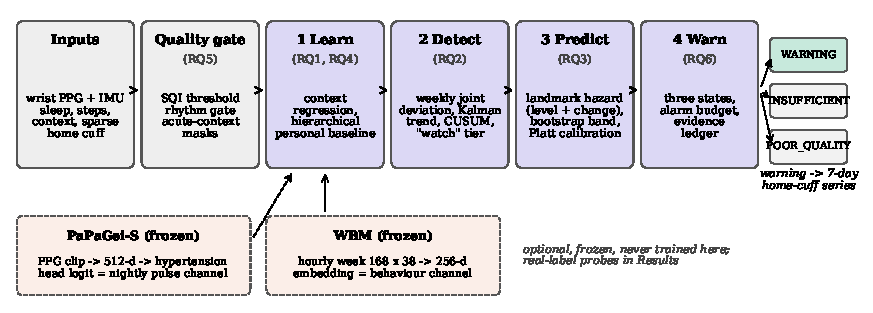
\includegraphics[width=\textwidth]{fig_architecture.pdf}
\caption{SENTINEL-HTN pipeline: quality gate, context-adjusted personal baselines (Learn), weighted joint weekly deviation with CUSUM, Kalman trend and a persistence ``watch'' tier (Detect), 26-week risk with a bootstrap band (Predict), and three states with an evidence ledger (Warn). A warning triggers home-cuff confirmation.}
\label{fig:arch}
\end{figure*}

\section{Experiments}
\subsection{Calibrated Simulator}
The organizers' data were unavailable, so we simulate people with a high-normal baseline BP ($116\pm5$/$72\pm3.5$\,mmHg). 35\% of them develop a 12--22\,mmHg systolic drift over 120--200 days. The confounders are season, illness, alcohol, exercise, menstrual cycles and firmware updates. About 26\% of days are missing, with extra loss for skin tone ITA$<$10$^\circ$, reflecting laboratory evidence \cite{mulholland2025}. Sparse 3-day cuff series define $t_{\mathrm{ref}}$, and about 16\% of people convert. Our first simulator used assumed noise. We then calibrated it on LifeSnaps, a public dataset of 71 people followed for about four months with a Fitbit Sense \cite{lifesnaps2022}. For every channel, the person mean, between-person SD, within-person SD and lag-1 autocorrelation now match the real data within about 10\%. For example, nocturnal HR has a within-person SD of 4.29 (real) against 4.28\,bpm (simulated), and Fitbit's smoothed resting HR has an autocorrelation of 0.88 against 0.90. The day-to-day noise is AR(1). The couplings to latent BP (e.g.\ $+0.15$\,bpm per mmHg) remain assumptions.

\subsection{Protocol and Metrics}
Each seed simulates 1,200 people over 540 days, split by subject into 60/20/20 fit, calibration and test sets. There are 39--45 test converters per seed, and we report mean$\pm$SD (sample) over three seeds. The metrics follow the challenge:
\begin{itemize}
\item (A) AUROC and AUPRC over landmarks;
\item (B) event-level sensitivity Se$_L$ for first warnings at least $L$ days before $t_{\mathrm{ref}}$, with abstention counted as a miss;
\item (C) warning episodes per non-converter person-year, and warning precision;
\item (D) Brier score and expected calibration error (ECE);
\item (E) test-only degradation;
\item (F) risk--coverage and abstention.
\end{itemize}
Because Se$_L$ credits any early warning, a \emph{chance floor} places random warnings at the model's own alarm rate. Ablations remove personalization or context, keep only level, cuff or change features, use equal channel weights, or drop the literature prior (reliability-only). Level-only and cuff-only are mandatory nulls. For the \emph{real-world transfer test}, the model and thresholds trained on simulation are applied to LifeSnaps. Only the label-free parts (context coefficients, population prior, channel weights, trend noise) are refitted. LifeSnaps has no BP labels, so we report coverage, abstention and alarm rates, with every participant treated as a non-converter.

\section{Results}
Table~\ref{tab:main} gives the held-out results. The full model reached an AUROC of $0.621\pm0.014$ and an AUPRC of $0.120\pm0.020$, exceeding every ablation in every seed except change-only (0.620 and 0.121), which it matched. Weighting raised AUROC from 0.605 (equal weights) in every seed. Reliability weighting alone (0.609), however, gave little gain, so most of the improvement comes from the literature prior. The simulator's couplings encode the same physiological beliefs, so this gain shows the mechanism works if the prior is right; only labelled real data can show that it is. Removing personalization or context cut AUROC to 0.567 and 0.550. Calibration was good (Brier $0.059\pm0.004$, ECE $0.006\pm0.004$; Fig.~\ref{fig:outcomes}a), with $0.41\pm0.04$ alarms per non-converter person-year and a warning precision of $0.209\pm0.010$.\n\n\begin{table}[t]
\centering
\caption{Held-out results on the calibrated simulator (mean$\pm$SD, three seeds). Se$_{30}$/Se$_{90}$: converters first warned $\geq$30/90 days before $t_{\mathrm{ref}}$. Alarms: warning episodes per non-converter person-year. Chance: random warnings at the full model's alarm rate.}
\label{tab:main}
\setlength{\tabcolsep}{2.5pt}
\footnotesize
\resizebox{\columnwidth}{!}{%
\begin{tabular}{@{}lccccc@{}}
\toprule
Model & AUROC & AUPRC & Se$_{30}$ & Se$_{90}$ & Alarms \\
\midrule
\textbf{Full} & \textbf{.621$\pm$.014} & \textbf{.120$\pm$.020} & \textbf{.322$\pm$.051} & .161$\pm$.072 & .405$\pm$.036 \\
Equal weights & .605$\pm$.024 & .104$\pm$.020 & .248$\pm$.084 & .105$\pm$.040 & .360$\pm$.101 \\
Reliability only & .609$\pm$.021 & .107$\pm$.020 & .249$\pm$.122 & .130$\pm$.080 & .360$\pm$.141 \\
Level-only (null) & .537$\pm$.033 & .070$\pm$.007 & .124$\pm$.122 & .083$\pm$.086 & .174$\pm$.152 \\
Cuff-only (null) & .545$\pm$.020 & .074$\pm$.005 & .149$\pm$.137 & .099$\pm$.111 & .236$\pm$.188 \\
Change-only & .620$\pm$.007 & .121$\pm$.015 & .324$\pm$.083 & .154$\pm$.037 & .456$\pm$.107 \\
No personaliz. & .567$\pm$.038 & .083$\pm$.019 & .190$\pm$.048 & .120$\pm$.009 & .372$\pm$.041 \\
No context & .550$\pm$.022 & .078$\pm$.010 & .193$\pm$.046 & .138$\pm$.043 & .357$\pm$.054 \\
\midrule
Chance & -- & -- & .254$\pm$.021 & .204$\pm$.018 & .405 \\
\bottomrule
\end{tabular}}
\end{table}

Early detection beat chance at 30 days but not at 90. At the model's own alarm rate, random warnings reached Se$_{30}=0.254$ and Se$_{90}=0.204$. The full model reached $0.322\pm0.051$ at 30 days, above chance in every seed. At 90 days it reached $0.161\pm0.072$, above chance in only one seed. The baselines stayed at or below chance. Of 125 test converters, 60 (48\%) were warned before $t_{\mathrm{ref}}$, with a median lead of $61\pm9$ days (Fig.~\ref{fig:outcomes}b). The operating curve agrees: at 1 alarm per person-year, Se$_{90}$ was 0.282 against 0.428 for chance. On the uncalibrated simulator, an earlier version had appeared to warn 48\% of converters 30 days ahead. Most of that advantage came from optimistic, independent day-to-day noise, and it shrank once real autocorrelated noise was modelled. The claim we retain is therefore modest: about a month of lead over chance, not three months.\n\n\begin{figure}[t]
\centering
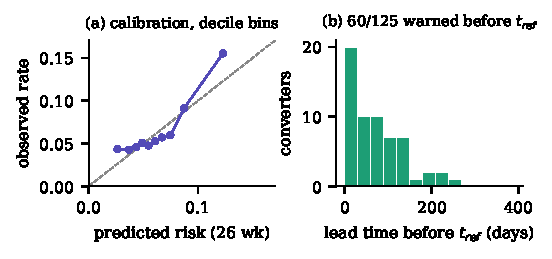
\includegraphics[width=\columnwidth]{fig_outcomes.pdf}
\caption{(a) Calibration of the 26-week risk on pooled test landmarks. (b) Lead time of the first warning before $t_{\mathrm{ref}}$ for converters warned beforehand (three seeds pooled).}
\label{fig:outcomes}
\end{figure}

Under test-only degradation (Fig.~\ref{fig:robust}a), AUROC stayed between 0.56 and 0.60. Skin-tone-weighted missingness and sensor failure were absorbed by abstention (0.31 and 0.52) rather than by alarms (0.25 and 0.17 per person-year). Additive noise, which the SQI cannot see, raised alarms to 0.72. Across skin-tone terciles (Fig.~\ref{fig:robust}b), the darkest tercile had higher abstention (0.234 against 0.045 in the lightest), a lower AUROC (0.584 against 0.651) and a lower Se$_{30}$ (0.210 against 0.409), a substantial equity gap.\n\n\begin{figure}[t]
\centering
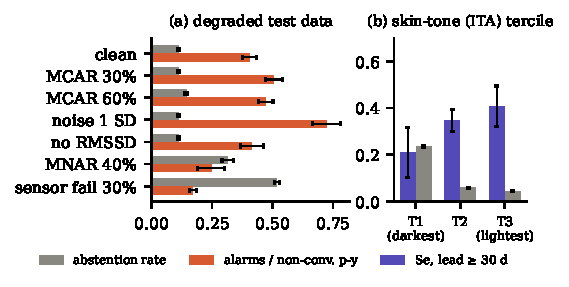
\includegraphics[width=\columnwidth]{fig_robustness.pdf}
\caption{(a) Abstention and alarm burden with degraded test data (models fitted on clean data). (b) Se$_{30}$ and abstention by skin-tone tercile. Error bars: SD over three seeds.}
\label{fig:robust}
\end{figure}

Table~\ref{tab:rw} reports the real-world transfer test. Only 49 of the 71 LifeSnaps participants reached a ready baseline within their median 87-day follow-up. Nocturnal HR and HRV were present on 58\% of valid days, and only 25\% of weeks were evaluable, against 71\% in simulation. Real weekly deviation was noisier (SD 0.41 against 0.30), and channel weighting reduced it from 0.52 with equal weights. Over 8.3 person-years, the system issued no warnings, which gives a 95\% upper bound of 0.36 false-alarm episodes per person-year. It abstained in 23\% of weeks, and the sparse weeks rarely satisfied the persistence rule. The low alarm rate therefore reflects abstention as much as specificity.

\begin{table}[t]
\centering
\caption{Real-world transfer test: LifeSnaps (Fitbit, no BP labels) vs simulated non-converters, same model and thresholds.}
\label{tab:rw}
\footnotesize
\begin{tabular}{@{}lcc@{}}
\toprule
Metric & Simulated & LifeSnaps \\
\midrule
People with ready baseline / person-years & 200 / 273.5 & 49 / 8.3 \\
Valid days; nocturnal-HR coverage of valid days & .67; .64 & .67; .58 \\
Evaluable weeks & .71 & .25 \\
Weekly deviation SD (equal weights) & .30 (.37) & .41 (.52) \\
Abstention (weeks \textsc{Poor\_Quality}) & .11 & .23 \\
Watch / warning episodes per person-year & 1.10 / .48 & .48 / .00 \\
\bottomrule
\end{tabular}
\end{table}

\section{Limitations}
All discrimination results are simulated. Noise is now calibrated to real wearables, but the couplings between physiology and BP, the drift time course and the labels are assumptions, so only the organizers' data can establish performance. The real cohort provides no labels and short follow-up. The simulator also compresses drift into months, whereas real hypertension develops over years. Our clearest negative finding is that warning 90 days ahead did not beat chance under realistic noise. The system's honest claim is a calibrated risk with about a month of lead, not months. Precision (0.21) is below the 0.30 a clinician would expect from a notification product, and enriching the enrolled population is the main lever. Further gaps remain:
\begin{itemize}
\item The channel prior comes from the literature, which the simulator's couplings also follow, so its simulated gain is partly circular. The organizers' labels should be used to confirm or re-estimate it, without tuning on the test split.
\item Additive noise inflates alarms, which calls for a noise-aware SQI.
\item The equity gap in darker skin reproduces a known limitation of optical sensing \cite{mulholland2025}. The cuff fallback mitigates it but does not remove it.
\item Obstructive sleep apnoea could masquerade as drift and should be screened.
\end{itemize}
Electromagnetic sensing is limited to a rhythm gate. ECG--PPG pulse arrival time is confounded by the pre-ejection period, which halves under physical stress \cite{pilz2023}, and radar pulse transit time has been validated in only 25 seated, individually calibrated participants \cite{zhu2026}. SENTINEL-HTN outputs no BP value, makes no diagnosis and makes no claim about acute events.

\section{Conclusion}
SENTINEL-HTN turns sparse, noisy data from one strap into a calibrated, evidence-backed prompt to measure BP, and it abstains when evidence is weak. With its simulator calibrated on real wearable data and its channels weighted by evidence and reliability, it beat level-only and cuff-only baselines on discrimination. It warned about a month earlier than chance, and its calibration was good. Calibration against real data also showed that an optimistic simulator had overstated the lead time, and it exposed a failure mode we fixed. We consider this, together with a label-free real-world test, the most credible contribution we can offer before the organizers' data are available. The code, data contract, LifeSnaps adapter and evaluation harness are released so these claims can be tested directly.\n\n\begin{thebibliography}{99}\footnotesize
\bibitem{staplin2023} N. Staplin \emph{et al.}, ``Relationship between clinic and ambulatory blood pressure and mortality: an observational cohort study in 59\,124 patients,'' \emph{Lancet}, vol. 401, pp. 2041--2050, 2023, doi: 10.1016/S0140-6736(23)00733-X.
\bibitem{esh2022} G. S. Stergiou \emph{et al.}, ``Cuffless blood pressure measuring devices: review and statement by the European Society of Hypertension Working Group on Blood Pressure Monitoring and Cardiovascular Variability,'' \emph{J. Hypertens.}, vol. 40, no. 8, pp. 1449--1460, 2022, doi: 10.1097/HJH.0000000000003224.
\bibitem{stergiou2023} G. S. Stergiou \emph{et al.}, ``European Society of Hypertension recommendations for the validation of cuffless blood pressure measuring devices,'' \emph{J. Hypertens.}, vol. 41, no. 12, pp. 2074--2087, 2023, doi: 10.1097/HJH.0000000000003483.
\bibitem{aha2026} J. B. Cohen \emph{et al.}, ``Cuffless devices for the measurement of blood pressure: a scientific statement from the American Heart Association,'' \emph{Hypertension}, vol. 83, no. 3, 2026, doi: 10.1161/HYP.0000000000000254.
\bibitem{mukkamala2023} R. Mukkamala \emph{et al.}, ``The Microsoft Research Aurora project: important findings on cuffless blood pressure measurement,'' \emph{Hypertension}, vol. 80, pp. 534--540, 2023, doi: 10.1161/HYPERTENSIONAHA.122.20410.
\bibitem{derendinger2024} F. C. Derendinger \emph{et al.}, ``Ability of a 24-h ambulatory cuffless blood pressure monitoring device to track blood pressure changes in clinical practice,'' \emph{J. Hypertens.}, vol. 42, pp. 662--671, 2024, doi: 10.1097/HJH.0000000000003667.
\bibitem{k250507} U.S. Food and Drug Administration, ``510(k) summary K250507: Hypertension Notification Feature, Apple Inc.,'' cleared Sep. 11, 2025.
\bibitem{cohen2026} J. B. Cohen \emph{et al.}, ``Impact of a smartwatch hypertension notification feature for population screening,'' \emph{JAMA}, vol. 335, no. 11, pp. 1001--1003, 2026, doi: 10.1001/jama.2025.26925.
\bibitem{kang2022} J. Kang \emph{et al.}, ``Ten-second heart rate variability, its changes over time, and the development of hypertension,'' \emph{Hypertension}, vol. 79, no. 6, pp. 1308--1318, 2022, doi: 10.1161/HYPERTENSIONAHA.121.18589.
\bibitem{bouwmeester2025} T. A. Bouwmeester \emph{et al.}, ``Autonomic cardiac control independently predicts incident hypertension and systolic blood pressure in a multi-ethnic population: the HELIUS study,'' \emph{Eur. J. Prev. Cardiol.}, vol. 33, no. 7, pp. 1116--1124, 2026, doi: 10.1093/eurjpc/zwaf011.
\bibitem{master2022} H. Master \emph{et al.}, ``Association of step counts over time with the risk of chronic disease in the All of Us Research Program,'' \emph{Nat. Med.}, vol. 28, pp. 2301--2308, 2022, doi: 10.1038/s41591-022-02012-w.
\bibitem{zheng2024} N. S. Zheng \emph{et al.}, ``Sleep patterns and risk of chronic disease as measured by long-term monitoring with commercial wearable devices in the All of Us Research Program,'' \emph{Nat. Med.}, vol. 30, pp. 2648--2656, 2024, doi: 10.1038/s41591-024-03155-8.
\bibitem{sau2025} A. Sau \emph{et al.}, ``Artificial intelligence-enhanced electrocardiography for prediction of incident hypertension,'' \emph{JAMA Cardiol.}, vol. 10, no. 3, p. 214, 2025, doi: 10.1001/jamacardio.2024.4796.
\bibitem{alavi2022} A. Alavi \emph{et al.}, ``Real-time alerting system for COVID-19 and other stress events using wearable data,'' \emph{Nat. Med.}, vol. 28, pp. 175--184, 2022, doi: 10.1038/s41591-021-01593-2.
\bibitem{empana2022} J.-P. Empana \emph{et al.}, ``Incidence of sudden cardiac death in the European Union,'' \emph{J. Am. Coll. Cardiol.}, vol. 79, no. 18, pp. 1818--1827, 2022, doi: 10.1016/j.jacc.2022.02.041.
\bibitem{fiorina2025} L. Fiorina \emph{et al.}, ``Near-term prediction of sustained ventricular arrhythmias applying artificial intelligence to single-lead ambulatory electrocardiogram,'' \emph{Eur. Heart J.}, vol. 46, no. 21, pp. 1998--2008, 2025, doi: 10.1093/eurheartj/ehaf073.
\bibitem{esc2024} J. W. McEvoy \emph{et al.}, ``2024 ESC Guidelines for the management of elevated blood pressure and hypertension,'' \emph{Eur. Heart J.}, 2024, doi: 10.1093/eurheartj/ehae178.
\bibitem{liu2025} H. Liu \emph{et al.}, ``Short-term effects of personal-level environmental temperature on ambulatory blood pressure in patients with hypertension: a multicity panel study,'' \emph{J. Am. Heart Assoc.}, vol. 14, no. 20, e045295, 2025, doi: 10.1161/JAHA.125.045295.
\bibitem{mulholland2025} A. M. Mulholland \emph{et al.}, ``Influence of skin pigmentation on the accuracy and data quality of photoplethysmographic heart rate measurement during exercise,'' \emph{Eur. J. Appl. Physiol.}, vol. 126, no. 2, pp. 1057--1066, 2026, doi: 10.1007/s00421-025-05977-x.
\bibitem{lifesnaps2022} S. Yfantidou \emph{et al.}, ``LifeSnaps, a 4-month multi-modal dataset capturing unobtrusive snapshots of our lives in the wild,'' \emph{Sci. Data}, vol. 9, 663, 2022, doi: 10.1038/s41597-022-01764-x.
\bibitem{pilz2023} N. Pilz \emph{et al.}, ``The pre-ejection period is a highly stress dependent parameter of paramount importance for pulse-wave-velocity based applications,'' \emph{Front. Cardiovasc. Med.}, vol. 10, 1138356, 2023, doi: 10.3389/fcvm.2023.1138356.
\bibitem{zhu2026} J. Zhu \emph{et al.}, ``Measuring multi-site pulse transit time with an AI-enabled mmWave radar,'' \emph{Nat. Commun.}, vol. 17, 4554, 2026, doi: 10.1038/s41467-026-73453-x.
\end{thebibliography}

\end{document}
